\documentclass[11pt]{article}
\usepackage[utf8]{inputenc}
\usepackage[letterpaper, total={6in, 9in}]{geometry}
\usepackage[table,xcdraw]{xcolor}
\usepackage{hyperref}
\usepackage{adjustbox,lipsum}

\usepackage{booktabs}
\usepackage{float}
\usepackage{tabularx}
\usepackage{hyperref}
\hypersetup{
    colorlinks,
    citecolor=black,
    filecolor=black,
    linkcolor=red,
    urlcolor=blue
}
\usepackage[round]{natbib}

\graphicspath{ {Assets/} }

\title{SE 3XA3: Software Requirements Specification\\Sudoku Solver}

\author{Team 08, SudoCrew
		\\ Rashad A. Bhuiyan (bhuiyr2)
		\\ Kai Zhu (zhuk2)
		\\ Stanley Chan (chans67)
}

\date{\today}

\begin{document}

\maketitle

\pagenumbering{roman}
\tableofcontents
\listoftables
\listoffigures

\begin{table}[bp]
\caption{\bf Revision History}
\begin{tabularx}{\textwidth}{p{3cm}p{2cm}X}
\toprule {\bf Date} & {\bf Version} & {\bf Notes}\\
\midrule
2022-02-07 & 0.0 & Drafted section 1\\
2022-02-09 & 0.1 & Completed sections 1, 2, and 4\\
2022-02-10 & 0.2 & Completed section 3\\
\bottomrule
\end{tabularx}
\end{table}

\newpage

\pagenumbering{arabic}

This document describes the requirements for a Sudoku Solver.  The template for the Software
Requirements Specification (SRS) is a subset of the Volere
template~\citep{RobertsonAndRobertson2012}.  If you make further modifications
to the template, you should explicity state what modifications were made.

\section{Project Drivers}

\subsection{The Purpose of the Project}
The purpose of this software application is to provide a comprehensive suite of tools for generating, recognizing, and solving Sudoku puzzles. The application will provide a web-based front-end with an intuitive interface to cater to users of different technical abilities on most modern hardware. Computer vision is also utilized to improve ease of use, by directly interfacing puzzles from print-media to the application.

\subsection{The Stakeholders}
\subsubsection{The Client}
The client of the project are the instructor, Dr. Asghar Bokhari, and teaching assistants of SFWRENG 3XA3. The clients stipulate the content and deadlines of the deliverables.

\subsubsection{The Customers}
The customers are any individuals with an interest in Sudoku. These includes hobbyists who seek to play the game or verify their solutions. The application is suitable for all demographics who can operate a web browser.

\subsubsection{Other Stakeholders}
Other stakeholders of the project include math teachers who may print generated puzzles from the application to use in educational setting. Tim Ruscica, the original developer of the open source Sudoku GUI Solver upon which this project is based on, also has a stake in seeing the expansion of features that stem from his work. Additionally, members of the SudoCrew development team are also stakeholders responsible for implementing and testing the application.

\subsection{Mandated Constraints}
\subsubsection{Solution Design Constraints}
\textbf{Description}: The game must operate on any browser with JavaScript enabled.
\\
\textbf{Rationale}: Potential users of the game will have access to a browser that can render JavaScript elements.
\\
\textbf{Fit Criterion}: The game will be made to operate on any browser with JavaScript enabled.

\subsubsection{Implementation Environment of the Current System}
N/A

\subsubsection{Partner or Collaborative Applications}
There are two main libraries used in the program: Flask and OpenCV. OpenCV is an API geared toward image recognition while Flask is a web framework that allows developers to build web applications using Python.

\subsubsection{Off-the-Shelf Software}
N/A

\subsubsection{Anticipated Workplace Environment}
The Internet with PC, laptop, mobile device, or tablet as a browsing device.

\subsubsection{Schedule Constraints}
\textbf{Description}: The project must follow the project schedule shown in the Tasks section.
\\
\textbf{Rationale}: The project must follow a predetermined plan in order to meet deliverable due dates on time.
\\
\textbf{Fit Criterion}: The project will follow the project schedule shown in the Tasks section.

\subsubsection{Budget Constraints}
N/A

\subsubsection{Enterprise Constraints}
N/A

\subsection{Naming Conventions and Terminology}
\begin{table}[H]
\caption{\bf Table of Naming Conventions and Terminology}
\centering
\begin{tabularx}{\textwidth}{p{3cm}X}
\toprule
Terminology     & Meaning \\
\midrule
UI     & User interface, the interface that allows for user interaction with the system. \\
Python & Language used for backend and frontend implementation through Flask.\\
HTML & Hypertext markup language, used to build websheets for the frontend part of the web application.\\
CSS & Cascading style sheets, used to style HTML files to make the application look more appealing.\\
JavaScript & Primary language used for scripting and functionality of the web application. \\
Git & The primary system for version control and code collaboration.\\
OpenCV & An open source computer vision library, and serves as the main Python library that will be used to detect Sudoku boards. \\
Pytest & A Python library designed to help create tests for Python code. \\
Pydoc & A Python library used to generate documentation for Python code. \\
Flask & A micro web framework for Python, and will mainly be used to create our web application and handle requests from the web.\\
\bottomrule
\end{tabularx}
\end{table}
\subsection{Relevant Facts and Assumptions}

\subsubsection{Facts}

\begin{enumerate}
    \item The original repository for the existing Sudoku solver has approximately 500 lines of code spread across 3 Python files.
    \item The existing implementation solves only contains a single static Sudoku board and displays the solution as a plain-text output.
\end{enumerate}

\subsubsection{Assumptions}

\begin{enumerate}
    \item The user has a stable Internet connection to use the web application.
    \item The user knows the basic basic rules of Sudoku.
    \item If the image upload option is to be used, the user has a legible photo of the whole puzzle board.
\end{enumerate}

\section{Functional Requirements}

\subsection{The Scope of the Work and the Product}

\subsubsection{The Context of the Work}
\begin{figure}[H]
    \centering
    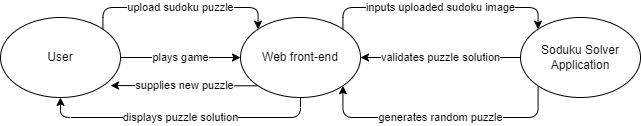
\includegraphics[width=\textwidth]{sudoku_scope}
    \caption{Work Context Diagram}
    \label{fig:my_label}
\end{figure}

The user either uploads a manually inputted or photographed Sudoku to receive feedback on a valid solution, or plays the game on a randomly generated puzzle grid. The Web front-end handles user input and interactive game-play while passing and receiving solution data to the back-end solver application.

\subsubsection{Work Partitioning}
\begin{table}[H]
\caption{\bf Table of Work Partitioning Events}
\label{tab:my-table}
\resizebox{\textwidth}{!}{%
\begin{tabular}{|c|l|l|l|}
\hline
\textbf{Event Number} & \multicolumn{1}{c|}{\textbf{Event Name}} & \multicolumn{1}{c|}{\textbf{Input}} & \multicolumn{1}{c|}{\textbf{Output}} \\ \hline
1 & Arrives at Homepage     & Mouse          & Webpage Generation   \\ \hline
2 & Uploading a sudoku board through an image     & Mouse          & Sudoku Board Solution   \\ \hline
3 & Uploading a sudoku board through manual input & Keyboard/Mouse & Sudoku Board Solution   \\ \hline
4 & Start a game of Sudoku                        & Mouse          & Sudoku Board Generation \\ \hline
\end{tabular}%
}
\end{table}

\newpage

\subsubsection{Individual Product Use Cases}
\begin{figure}[H]
    \centering
    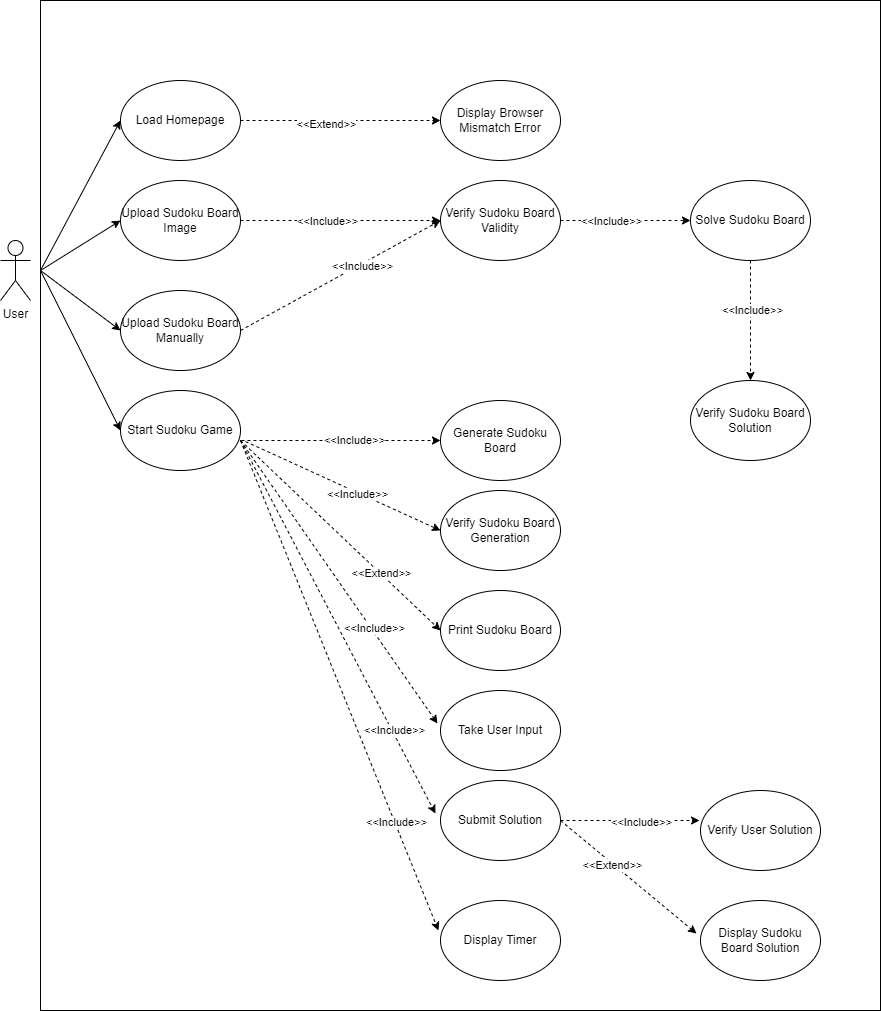
\includegraphics[width=\textwidth]{use_case}
    \caption{Use Case Diagram}
    \label{fig:my_label}
\end{figure}
The use case diagram above shows the various ways a user can interact with our web application. Since Starting a Sudoku game involves multiple game-play actions itself, it has a lot of included use cases. Furthermore, there are multiple levels of extends cases when verifying and sudoku board solutions as each complex use case is broken into simpler cases.
\newpage

\subsection{Functional Requirements}

\begin{enumerate}
    \item [BE1.] The user arrives at the main application portal (homepage)
    \begin{enumerate}
        \item [FR1.] The system must display links to play or get solution for a Sudoku game.
        \item [FR2.] The system shall display options for manual input or photo upload for the Sudoku solver.
        \item [FR3.] The system shall display an error if user browser is incompatible with the application.
    \end{enumerate}
    \item [BE2.] The user uploads a Sudoku board through an image
    \begin{enumerate}
        \item [FR4.] The system shall display a loading indicator to the user to show that their picture is being uploaded and solved.
        \item [FR5.] The system shall attempt to interpret the uploaded picture as a 9x9 Sudoku board modelled as an array.
        \item [FR6.] If the system fails to interpret a 9x9 Sudoku board from the uploaded image, the system must inform the user that the picture could not be interpreted.
        \item [FR7.] The system shall input the 9x9 array into the Sudoku solver algorithm to solve the Sudoku board.
        \item [FR8.] If the system finds a solution to the Sudoku board, the system shall display the solution in the user interface.
        \item [FR9.] If the system does not find a solution, the system must notify the user that the Sudoku board is invalid.
    \end{enumerate}
    \item [BE3.] The user uploads a Sudoku board through manual input
    \begin{enumerate}
        \item [FR10.] The system shall display an empty Sudoku grid
        \item [FR11.] The system must allow the user to type numbers 1 to 9 into the grid.
        \item [FR12.] The system must immediately notify the user of invalid input, including repeated numbers in a row, column, or subgrid.
        \item [FR13.] The system shall attempt to solve an outwardly valid board.
        \item [FR14.] If the system fails to find a solution to the input board, it must inform the user that the puzzle has no solution.
        \item [FR15.] If the system finds a solution, it must display the solution to the user through the user interface.
    \end{enumerate}
    \item [BE4.] The user starts a game of Sudoku
    \begin{enumerate}
        \item [FR16.] The system must generate a random valid Sudoku board.
        \item [FR17.] The system must output the generated Sudoku board to the user through the user interface.
        \item [FR18.] The system shall allow the user to print the generated puzzle.
        \item [FR19.] The system shall allow the user to type numbers into empty cells on the Sudoku board.
        \item [FR20.] The system must reject invalid user input (non-digits, repeated numbers on row, column, or subgrid) and notify user of the error.
        \item [FR21.] The system shall allow the user to submit the puzzle once all grid cells are filled.
        \item [FR22.] The system shall validate the submitted solution and display whether the solution is correct.
        \item [FR23.] The system shall display a timer to track the duration from puzzle generation to the submission of a correct solution.
    \end{enumerate}
\end{enumerate}

\section{Non-functional Requirements}

\subsection{Look and Feel Requirements}

\subsubsection{Look Requirements}

\begin{enumerate} % fill in the look/feel requirement number (LF#.)
    \item [LF1.] The system should display to the user an option to choose between uploading a Sudoku board, manually inputting a Sudoku board, or generating a random Sudoku board.
\end{enumerate}

\subsubsection{Feel Requirements}

\begin{enumerate} % fill in the look/feel requirement number (LF#.)
    \item [LF2.] The system should have a sleek and non-cluttered user interface.
    \item [LF3.] The user interface should have colours that are appealing and is accessible to people with potential colour blindness.
\end{enumerate}

\subsection{Usability and Humanity Requirements}

\subsubsection{Ease of Use Requirements}

\begin{enumerate}
    \item [UH1.] The system should be able to accept Sudoku boards from a variety of different mediums.
\end{enumerate}

\subsubsection{Ease of Learning Requirements}

N/A

\subsubsection{Accessibility Requirements}

\begin{enumerate}
    \item [UH2.] The colour palette must be accessible to users with colour blindness.
\end{enumerate}

\subsection{Performance Requirements}

\subsubsection{Speed Requirements}

\begin{enumerate}
    \item [PR1.] Upload of pictures to the system should take a maximum of \emph{MAX\_UPLOAD\_TIME} seconds. % feel free to alter
    \item [PR2.] The system should be able to solve a given Sudoku board within a timeframe of \emph{MAX\_SOLUTION\_TIME} seconds. % feel free to alter
\end{enumerate}

\subsubsection{Safety-Critical Requirements}

N/A

\subsubsection{Precision Requirements}

\begin{enumerate}
    \item [PR3.] The system should output the proper solution to the inputted Sudoku board.
    \item [PR4.] The system should accurately determine whether or not a given Sudoku board is valid.
\end{enumerate}

\subsubsection{Reliability and Availability Requirements} % don't think we will be hosting it on a web server?

N/A

\subsubsection{Capacity Requirements} % don't need storage or anything

N/A

\subsection{Operational and Environmental Requirements}

N/A

\subsection{Maintainability and Support Requirements} % don't need to maintain anything

N/A

\subsection{Security Requirements}

\subsubsection{File Integrity Requirements}

\begin{enumerate}
    \item [SR1.] Uploaded pictures should be deleted by the system after used by the Sudoku Solver.
\end{enumerate}

\subsubsection{Access Requirements}

N/A

\subsubsection{Privacy Requirements}

\begin{enumerate}
    \item [SR2.] Uploaded pictures should not be accessible to any user other than the system itself.
\end{enumerate}

\subsubsection{Audit Requirements}

N/A

\subsubsection{Immunity}

N/A

\subsection{Cultural Requirements}

\begin{enumerate}
    \item [CR1.] The user interface should not display any culturally insensitive imagery.
\end{enumerate}

\subsection{Legal Requirements}

N/A

\subsection{Health and Safety Requirements}

N/A

\section{Project Issues}

\subsection{Open Issues}
Sudoku recognition with computer vision may constitute a major challenge due to the large variety of factors that can affect image recognition, such as photo resolution, sharpness, exposure, angle, and colour balance. 

The image upload feature may also expose the system to potential attacks in the form of malicious file content.

\subsection{Off-the-Shelf Solutions}
OpenCV provides a suite of image processing functions such as adaptive thresholding and colour conversion that can be used to preprocess uploaded photos and improve their recognizability. 

\subsection{New Problems}
Higher traffic to the web application and the increased calls to the image recognizer and solver may increase the load on the system and potentially delay response times or cause crashes.

\subsection{Tasks}
Task schedules and delegated responsibilities are outlined in the project \href{https://gitlab.cas.mcmaster.ca/bhuiyr2/sudokusolver_l02_grp08/-/blob/main/ProjectSchedule/Gantt_Sudoku.pdf}{Gantt Chart}.

\subsection{Migration to the New Product}
The project will initially be hosted on GitLab and migrate to a hosting service such as Heroku for deployment of the proof-of-concept and final product.

\subsection{Risks}
The application does not collect user information and so does not expose users to data security risks. As a web application, the main risk to the system are higher-than-expected traffic overwhelming the system through high processing load, or malicious attacks including denial-of-service and viral uploads.

\subsection{Costs}
The project does not involve monetary cost as it uses only open-source resources. A labour cost of between 5-10 hours per week is expected from each group member during the development period outlined in the \href{https://gitlab.cas.mcmaster.ca/bhuiyr2/sudokusolver_l02_grp08/-/blob/main/ProjectSchedule/Gantt_Sudoku.pdf}{Gantt Chart}.

\subsection{User Documentation and Training}
\subsubsection{Documentation}
Basic instructions and rules of Sudoku will be outlined in the game interface. The user interface will also inform the user of any errors and provide remedy instructions, such as in the case of an unrecognizable photo, invalid input, or unsolvable uploaded puzzle.

\subsubsection{Training}
No training is required to use this application beyond the basic knowledge of using a web browser.

\subsection{Waiting Room}
Additional quality-of-life features, given extra development time, may include:
\begin{enumerate}
    \item Account system that saves player statistics such as solved puzzles and past uploads.
    \item Multiplayer challenge system that pits two players against each other on the same puzzle to improve the fun, competitive aspect of the game.
\end{enumerate}


\subsection{Ideas for Solutions}
N/A

\bibliographystyle{plainnat}

\bibliography{SRS}

\newpage

\section{Appendix}

This section has been added to the Volere template.  This is where you can place
additional information.

\subsection{Symbolic Parameters}

The definition of the requirements will likely call for SYMBOLIC\_CONSTANTS.
Their values are defined in this section for easy maintenance.\\

\noindent \emph{MAX\_UPLOAD\_TIME} = 3\\
\emph{MAX\_SOLUTION\_TIME} = 2

\end{document}